\chapter{Systême masse-ressort}
   \subsection{Modélisation}
      On considère un objet de masse \(m\) relié à un mur par un ressort de longueur \(l\), tous deux des réels positifs. On considère aussi que la masse est à l'équilibre, voici un schéma qui illustre la situation:
      \begin{center}
         \begin{tikzpicture}[>=stealth]
            \path[pattern={Lines[angle=45,distance={8pt/sqrt(2)}]}] (-2,5) edge ++(4,0)
            rectangle ++ (4,0.5);
            \draw[decorate,decoration={coil,segment length=5pt,aspect=0.7,amplitude=4pt,
               pre=lineto,pre length=3mm,post=lineto,post length=3mm},thick] (0,5) -- (0,2.5)
               node[below,draw,minimum size=1cm,fill=DarkGreen1!50](m){$m$};

            \draw[<->, DarkGreen3] (-0.5,4.96) -- node[left=1mm] {$l$} (-0.5, 2.54);

            \draw[DarkGreen3] (m.east) edge[dashed] (m.east-|2,0) (m.east-|2,0) node[right] {Equilibre};
         \end{tikzpicture}
      \end{center}
   Le système qu'on cherche à modéliser est le mouvement de la masse si on déplace la masse en dehors du point d'équilibre. On peut tout d'abord identifier les \textbf{paramétres du modèle}:
   \begin{itemize}
      \item La masse de l'objet.
      \item La longeur du ressort.
      \item La force de gravité.
   \end{itemize}
   Aussi, on peut remarque que si quand la masse est à l'équilibre et si on note \(l_0\) la longueur du ressort à vide, alors la force de gravité est proportionelle à l'élongation du ressort, ie on a:
   \[
      mg = k(l - l_0)
   \]
   On appelle alors \(k\) la \textbf{constante de raideur} du ressort. Notons \(y\) la fonction qui donne la position au temps \(t\) du centre de la masse. Pour modéliser le mouvement de la masse si on la sort de la position d'équilibre, on doit modéliser les forces en action.  D'aprés la 3em loi de Newton, on a la situation suivante:
   \begin{center}
      \begin{tikzpicture}[>=stealth]
         \path[pattern={Lines[angle=45,distance={8pt/sqrt(2)}]}] (-2,5) edge ++(4,0)
         rectangle ++ (4,1);
         \draw[decorate,decoration={coil,segment length=7pt,aspect=0.7,amplitude=4pt,
            pre=lineto,pre length=3mm,post=lineto,post length=3mm},thick] (0,5) -- (0,2.02)
            node[below,draw,minimum size=1cm,fill=DarkGreen1!50](m){$m$};

         \draw[dashed, DarkGreen3] (0.5,2) -- node[right=5mm]{Equilibre} (1.5, 2);
         \draw[->, thick, DarkGreen3] (0,1) -- node[right]{$\vv{F}$} (0, 0.30);
         \draw[->, thick, BrightRed2] (0,5.0) -- node[right]{$\vv{F}$} (0, 5.70);
      \end{tikzpicture}
   \end{center}
   \pagebreak
   En effet gràce à la relation de proportionnalité ci-dessus, la gravité n'a pas d'impact sur le mouvement du ressort, elle ne fait que déplacer le point d'équilibre vers le bas. En outre, la force qu'exercerce le ressort dans la direction de l'équilibre est donc linéairement proportionelle à la distance avec l'équilibre, et donc d'aprés le \textbf{principe fondamental de la dynamique}, ie on a:
   \[
      \vv{a}(t) = \frac{1}{m}\sum \vv{F}(t)
   \]
   Et donc on obtient en faisant le bilan des forces, dont il ne resulte qu'une force proportionnelle à l'élongation:
   \[
      \boxed{y''(t) = -\frac{k}{m}y(t)}
   \]
   Cette équation modélise donc bien le mouvement de la masse sur le ressort.
   \subsection{Résolution}
      L'équation précédente et facilement résoluble, en effet c'est une equation linéaire et on peut remarquer facilement que les fonctions solutions sont de la forme:
      \[
         y(t) = c_1\cos(\omega t) + c_2\sin(\omega t) \; ; \; \omega = \sqrt{\frac{k}{m}}
      \]
      Où \(c_1, c_2\) sont les constantes d'intégration à déterminer, on a:
      \begin{itemize}
         \item On a directement \(y(0) = c_1\) donc \(c_1\) est la position initale de la masse.
         \item On a en dérivant que \(y'(0) = \omega c_2\), donc \(c_2 = \frac{v_0}{\omega}\), c'est une constante proportionelle à la vitesse initiale.
      \end{itemize}
      Finalement on a la solution donnée par:
      \[
         \boxed{y(t) = y_0\cos(\omega t) + \frac{v_0}{\omega}\sin(\omega t) \; ; \; \omega = \sqrt{\frac{k}{m}}}
      \]
   \subsection{Champ de vecteur associé et portrait de phase}
      Si on ramène l'équation différentielle d'ordre 2 à une équation différentielle vectorielle d'ordre 1, on obtient que le mouvement de la masse est exactement caractérisé par sa position et sa vitesse, ie l'espace des phases est le plan repéré par \((y, y')\), et la dynamique est caractérisée par le champ de vecteur associé trouvé ci-dessus. Par exemple pour \(k = 1\), on a le champ de vecteur suivant:
      \begin{center}
         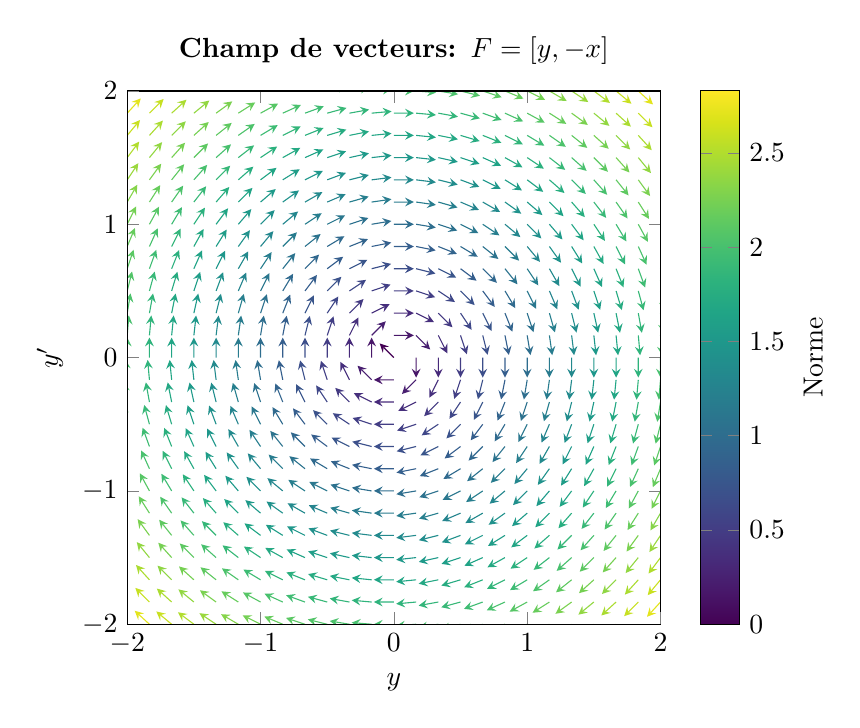
\begin{tikzpicture}
            \begin{axis}[
               xmin = -2, xmax = 2,
               ymin = -2, ymax = 2,
               zmin = 0, zmax = 1,
               axis equal image,
               xtick distance = 1,
               ytick distance = 1,
               view = {0}{90},
               scale = 1.25,
               title = {\bf Champ de vecteurs: $F = [y,-x]$},
               height=7cm,
               xlabel = {$y$},
               ylabel = {$y'$},
               colormap/viridis,
               colorbar,
               colorbar style = {
                  ylabel = {Norme}
               }
            ]
               \addplot3[
                  point meta = {sqrt(x^2+y^2)},
                  quiver = {
                     u = {y/sqrt(x^2+y^2)},
                     v = {-x/sqrt(x^2+y^2)},
                     scale arrows = 0.15,
                  },
                  quiver/colored = {mapped color},
                  -stealth,
                  domain = -2:2,
                  domain y = -2:2,
               ] {0};   
            \end{axis}
         \end{tikzpicture}
      \end{center}

      \pagebreak
      
      Traçons quelques trajectoires possibles du système, pour les conditions initiales \((y_0, v_0) = (\frac{i}{2}, 0)\) pour \(i \in \{1, 2, 3\}\), on trouve les trajectoires suivantes:

      \begin{center}
         \begin{tikzpicture}
            \tikzset{%
               my arrow/.style={
               postaction={decorate,decoration={
               markings,
               mark=between positions 0.25 and 1 step 0.15 with {\arrow[line width=1.5pt]{stealth}}}}
               }
            }
            \begin{axis}[
               xmin = -2, xmax = 2,
               ymin = -2, ymax = 2,
               zmin = 0, zmax = 1,
               axis equal image,
               xtick distance = 1,
               ytick distance = 1,
               view = {0}{90},
               scale = 1.25,
               title = {\bf Portrait de phase: $F = [y,-x]$},
               height=7cm,
               xlabel = {$y$},
               ylabel = {$y'$},
               colormap/viridis,
               colorbar,
               colorbar style = {
                  ylabel = {Norme}
               }
            ]
               \addplot3[
                  point meta = {sqrt(x^2+y^2)},
                  quiver = {
                     u = {y/sqrt(x^2+y^2)},
                     v = {-x/sqrt(x^2+y^2)},
                     scale arrows = 0.15,
                  },
                  quiver/colored = {mapped color!25},
                  -stealth,
                  domain = -2:2,
                  domain y = -2:2,
               ] {0};
               \addplot [my arrow, samples=100, domain=0:2*pi, line width = 1.1, postaction={decorate}] ( {0.5*cos(deg(x))}, {-0.5*sin(deg(x))});      
               \node[thick] at (axis cs:0.70, 0) {\Large $\gamma_1$};   
               \addplot [my arrow, samples=100, domain=0:2*pi, line width = 1.1, postaction={decorate}] ( {cos(deg(x))}, {-sin(deg(x))} );   
               \node[thick] at (axis cs:1.20, 0) {\Large $\gamma_2$};   
               \addplot [my arrow, samples=100, domain=0:2*pi, line width = 1.1, postaction={decorate}] ( {1.5*cos(deg(x))}, {-1.5*sin(deg(x))} );      
               \node[thick] at (axis cs:1.70, 0) {\Large $\gamma_3$};      
            \end{axis}
         \end{tikzpicture}
      \end{center}
      On remarque donc la propriété suivante:
      \begin{center}
         \textbf{Toutes les trajectoires sont périodiques et le seul point d'équilibre correspond à la masse au repos.}
      \end{center}
      La vitesse est la position sont alors deux fonctions périodiques élémentaires déphasées dont l'amplitude dépend de la vitesse/élongation initiale.
   \subsection{Ajout d'un terme d'amortissement}
      On essaie maintenant de rendre le modèle plus réaliste en ajoutant la contribution des frottements de l'air. Alors, en première approximation, on peut imaginer rajouter un terme linéaire, ie proportionnel à la vitesse, qui ralentit la masse. On considère alors la nouvelle équation suivante, pour \(\lambda > 0\) un coefficient de frottements:
      \[
         y''(t) = -\frac{k}{m}y(t) - \lambda y'(t)
      \]
      Par passage à une EDO d'ordre 1, on obtient facilement que le champs de vecteurs associé est:
      \[ 
         F(x, y) = \left(y, - \frac{k}{m}x - \lambda y \right)
      \]
      Pour illustrer la situation, on considère alors à nouveau le cas \( k=1 \) et \( \lambda = 0.5 \) et on obtient le portrait de phase suivant:
      \begin{center}
         \begin{tikzpicture}
            \tikzset{%
               my arrow/.style={
               postaction={decorate,decoration={
               markings,
               mark=between positions 0.25 and 1 step 0.15 with {\arrow[line width=1.5pt]{stealth}}}}
               }
            }
            \begin{axis}[
               xmin = -2, xmax = 2,
               ymin = -2, ymax = 2,
               zmin = 0, zmax = 1,
               axis equal image,
               xtick distance = 1,
               ytick distance = 1,
               view = {0}{90},
               scale = 1.25,
               title = {\bf Portrait de phase: $F = [y,-x - 0.5y]$},
               height=7cm,
               xlabel = {$y$},
               ylabel = {$y'$},
               colormap/viridis,
               colorbar,
               colorbar style = {
                  ylabel = {Norme}
               }
            ]
            \def\length{sqrt(y^2 + (-x - 0.5*y)^2)}
               \addplot3[
                  point meta = {\length},
                  quiver = {
                     u = {y/\length},
                     v = {(-x - 0.5*y)/\length},
                     scale arrows = 0.15,
                  },
                  quiver/colored = {mapped color!50},
                  -stealth,
                  domain = -2:2,
                  domain y = -2:2,
                  axis equal image
               ] {0};
               \addplot[mark = none, color = black!75] table {data/springMass/springMass1.dat}; 
               \node[thick] at (axis cs:0.70, 0) {\Large $\gamma_1$};   
               \addplot[mark = none, color = black!75] table {data/springMass/springMass2.dat};
               \node[thick] at (axis cs:1.20, 0) {\Large $\gamma_2$};   
               \addplot[mark = none, color = black!75] table {data/springMass/springMass3.dat};
               \node[thick] at (axis cs:1.70, 0) {\Large $\gamma_3$};      
            \end{axis}
         \end{tikzpicture}
      \end{center}   
      On peut aussi constater le comportement du systême en étudiant la fonction vitesse:
      \begin{center}
         \begin{tikzpicture}
            \tikzset{%
               my arrow/.style={
               postaction={decorate,decoration={
               markings,
               mark=between positions 0.25 and 1 step 0.15 with {\arrow[line width=1.5pt]{stealth}}}}
               }
            }
            \begin{axis}[
               xmin = 0, xmax = 6.2,
               ymin = -1.5, ymax = 1.5,
               zmin = 0, zmax = 1,
               xtick distance = 1,
               ytick distance = 1,
               view = {0}{90},
               scale = 1.25,
               title = {\bf Vitesse par unité de temps},
               height=7cm,
               xlabel = {$t$},
               ylabel = {$y'$},
            ]
            \addplot[mark = none, color = black!75] table {data/springMass/springMass3partialY.dat}; 
            \end{axis}
         \end{tikzpicture}
      \end{center}               
